\section{Dimensionless Boundary Validation}
\label{sec:boundary-results}

E15 completed all \EFifteenGridCount{} required grid cells and all \EFifteenSobolCount{} continuous holdouts. Every required cell satisfied the preregistered classification: configurations at $\rho\le0.95$ exhibited a rest-to-rest pulse fraction of at least $0.95$, and configurations at $\rho\ge1.05$ exhibited a pulse fraction of at most $0.05$. This agreement spans both signs, all four control periods, both jerk levels, and both branches of $g(q)$. The collapse in \cref{fig:e15-collapse} therefore supports the predicted dimensionless boundary for the tested implementation away from its deliberately excluded seam.\claimtag{C2}

The continuous holdout provides a more stringent threshold check than the coarse primary bands. Bisection recovered every Sobol threshold, and the maximum absolute error was \EFifteenMaxBoundaryErrorPercent{} in $\rho$. The residual is consistent with the finite ten-step bisection resolution: all recovered thresholds lie just above one by the same small fraction. This is a numerical threshold-recovery result, not statistical uncertainty. The 128 points are out-of-grid configurations, but they are not 128 physical systems or robot tasks.

\begin{figure*}[t]
 \centering
 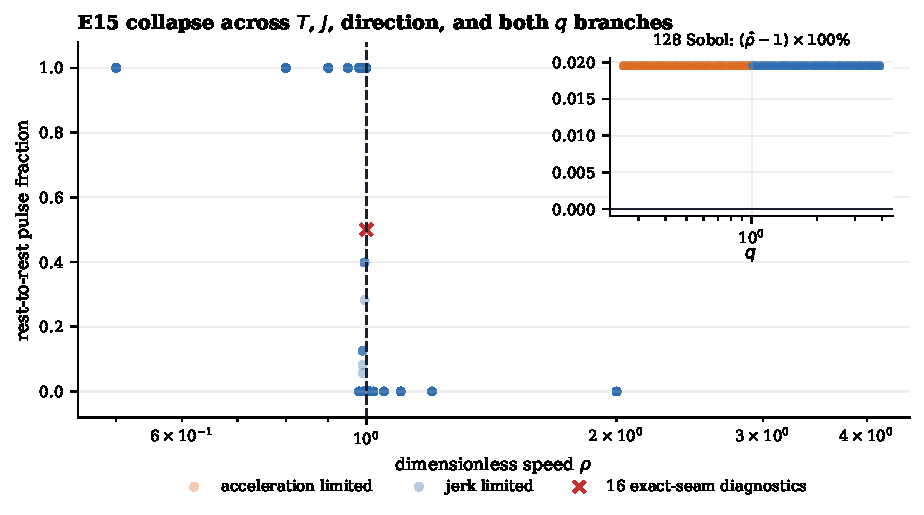
\includegraphics[width=\textwidth]{figures/generated/fig3_e15_collapse.pdf}
 \caption{E15 dimensionless collapse. Required cells from both analytic branches switch across $\rho=1$ after varying period, jerk, and direction. The red marker denotes 16 coincident exact-seam diagnostics, all of which produced native failures in Ruckig~\RuckigVersion. The inset shows the small positive error of all 128 Sobol threshold estimates.}
 \label{fig:e15-collapse}
\end{figure*}

The exact seam must be read differently. All \EFifteenSeamCount{} cells at $q=1,\rho=1$ produced a native solver failure. They are shown in \cref{fig:e15-collapse} rather than dropped. Because the analytic profile topology changes at $q=1$ and one-period feasibility is tight at $\rho=1$, this coordinate combines two boundaries. The experiment does not localize a software defect or prove that a deadband is mathematically necessary there. It establishes a reproducible numerical behavior of version \RuckigVersion{} at an exact seam. The required grid excludes these diagnostics by design, so their failure neither changes the theorem nor gets counted as successful boundary confirmation.

The phase map also clarifies why endpoint RMSE alone would be misleading. Below the boundary, many cells exactly reach the scheduled endpoint and report an exact profile, yet their pulse fraction and endpoint-stop fraction are one. Above the boundary, the one-period rest target is infeasible and the profile cannot complete the same repeated stop. The transition is thus about the reachable terminal state, not loss of position accuracy. This links the theory to the observed mechanism without treating the theorem as a statement about solver policy.\claimtag{C1}

Finally, the cross-limit collapse supports the monotonic implication in \cref{cor:monotonic}. The same physical reference speed can move from $\rho>1$ to $\rho<1$ when $A$, $J$, or $T$ increases. In the tested setting, such a change makes the unintended per-tick rest request reachable. This is why tuning limits can move the symptom while leaving its semantic cause untouched.

